\documentclass[conference]{IEEEtran}
\usepackage[T1]{fontenc}
\usepackage[utf8]{inputenc}
\IEEEoverridecommandlockouts
\usepackage{cite}
\usepackage{amsmath,amssymb,amsfonts}
\usepackage{graphicx}
\usepackage{textcomp}
\usepackage{xcolor}
\usepackage{booktabs}
\usepackage{multirow}
\usepackage{array}
\usepackage{hyperref}

\begin{document}

\title{Graph Neural Networks for Node and Graph Classification:\\
An Empirical Comparison Across Three Heterogeneous Datasets}

\author{
\IEEEauthorblockN{Adithya Nangarath\textsuperscript{1}, K V Nikhilesh\textsuperscript{2}, Vishruth Vijay\textsuperscript{3}}
\IEEEauthorblockA{\textsuperscript{1}IMT2022024\quad \textsuperscript{2}IMT2022511\quad \textsuperscript{3}IMT2022507\\
Graph Neural Networks Research Project}
}

\maketitle

\begin{abstract}
We present a systematic empirical comparison of three Graph Neural Network architectures---GAT, GraphSAGE, and GIN---across three fundamentally different graph-learning tasks: 10-class node classification on the Amazon Computers co-purchase graph (13,752 nodes), ordinal node regression on the USA Airports traffic network (1,190 nodes), and binary graph classification on OGBG-MOLHIV (41,127 molecular graphs). Our three primary contributions are: (1) a rigorous hyperparameter grid search yielding architecture-specific best configurations on each dataset; (2) a novel comparison of ordinal regression (MSELoss) versus classification (CrossEntropyLoss) formulations for the Airports task, showing that the ordinal loss eliminates 100\% of catastrophic regional-to-hub misclassifications (2.381 percentage points); and (3) ablation studies and t-SNE visualisations on MOLHIV confirming that both atom features and bond topology are indispensable for HIV inhibition prediction. GIN achieves the best overall rank across datasets (rank sum = 5), and leads on Airports ordinal regression with a weighted kappa of 0.5758$\pm$0.016.
\end{abstract}

% ─────────────────────────────────────────────────────────────────────────────
\section{Introduction}
% ─────────────────────────────────────────────────────────────────────────────

Graph Neural Networks (GNNs) have emerged as the dominant paradigm for learning on relational data, combining node feature representations with structural information through message passing \cite{gilmer2017}. Despite rapid architectural advances, rigorous comparative studies across tasks of fundamentally different character---node classification, ordinal regression, and graph-level binary classification---remain scarce. Practitioners must choose an architecture without clear empirical guidance tailored to their graph type.

This work addresses that gap through three concrete contributions. \textbf{First}, we conduct a controlled grid search (8 hyperparameter combinations per model per dataset) and report test-set performance with tuned configurations for GAT, GraphSAGE, and GIN alongside an MLP baseline, demonstrating that graph structure provides a 6.44 percentage-point accuracy gain over feature-only learning on Amazon. \textbf{Second}, we introduce an ordinal regression formulation for the USA Airports dataset, replacing the original CrossEntropyLoss with MSELoss on a scalar output to exploit the natural ordering of passenger-throughput quartiles; the quadratic penalty reduces catastrophic regional-to-hub misclassifications by 2.381 percentage points over the classification baseline. \textbf{Third}, on OGBG-MOLHIV---our largest dataset at 41,127 molecular graphs---we contribute ablation studies isolating atom-feature and bond-structure contributions, plus t-SNE visualisations with misclassification overlays for all three architectures.

We deliberately omit Graph Convolutional Networks (GCN) \cite{kipf2017} because GAT \cite{velickovic2018} strictly subsumes GCN: uniform attention weights in GAT reduce to GCN's normalised mean aggregation, making a separate GCN evaluation redundant.

% ─────────────────────────────────────────────────────────────────────────────
\section{Datasets and Task Definitions}

Table~\ref{tab:datasets} summarises the statistical properties of the three benchmark datasets used in this study, which differ substantially in scale (from 1,190 nodes to 41,127 graphs), feature semantics (sparse bag-of-words versus one-hot positional encodings versus domain-specific chemistry), and task definition (classification versus ordinal regression). To ensure robust evaluation, each dataset employs an appropriate splitting strategy: Amazon and Airports use stratified random splits to preserve class distributions, whereas MOLHIV uses a scaffold split to evaluate generalisation to unseen chemical structures.
% ─────────────────────────────────────────────────────────────────────────────

\subsection{Amazon Computers}

The Amazon Computers dataset \cite{shchur2018} is a co-purchase graph with 13,752 product nodes and 245,778 directed edges. Each node carries a 767-dimensional sparse bag-of-words feature vector derived from product reviews (sparsity 65.16\%). The task is 10-class node classification by product category.

Node features alone are insufficient: words such as ``DDR4'' and ``SATA'' appear in reviews for both laptops and desktop components, creating ambiguity that a feature-only MLP cannot resolve. Graph structure alone is equally insufficient: a product with ambiguous reviews cannot be classified from connectivity if its neighbours are drawn from multiple categories. Together, a generic carrying case co-purchased with laptops is assigned to Computer Accessories, while the same case co-purchased with cameras maps to Photo Accessories---structure resolves category ambiguity that features cannot.

\subsection{USA Airports}

The USA Airports dataset \cite{ribeiro2017} consists of 1,190 airport nodes and 13,599 undirected flight-route edges. Node features are 1,190-dimensional one-hot identity vectors (no semantic content), so graph-structural position is the \emph{only} transferable signal. Labels 0--3 encode passenger throughput quartiles (0 = major hub, 3 = regional).

A Spearman rank correlation of $\rho = -0.773$ ($p = 4.86 \times 10^{-237}$) between node degree and activity label confirms a strong monotonic relationship, justifying treatment of labels as an ordered scale. The negative sign reflects the struc2vec dataset's label encoding: in this dataset, higher node degree corresponds to lower label values (more connected airports receive smaller quartile indices), so the magnitude $|\rho|=0.773$ is what matters---structural position is strongly predictive of activity quartile regardless of encoding direction. Under CrossEntropyLoss the penalty for predicting class 0 when the true label is 3 equals the penalty for predicting class 2---the ordering is ignored. Under MSELoss on a scalar output, the squared errors are $(3-0)^2 = 9$ versus $(3-2)^2 = 1$, penalising large ordinal violations quadratically and giving the model a corrective gradient proportional to prediction severity.

\subsection{OGBG-MOLHIV}

OGBG-MOLHIV \cite{hu2020} contains 41,127 molecular graphs (our largest dataset) with binary labels indicating HIV inhibition ($\approx 3.5\%$ positive; $\text{pos\_weight} = 25.71$). Graphs use a scaffold split to ensure chemical diversity across train/val/test. Each node carries 9-dimensional atom features; each edge carries 3-dimensional bond features. Atom features (pharmacophore identity) and bond topology (3-D geometric fit to the HIV enzyme pocket) are both necessary: atom type determines binding potential while bond structure determines whether the 3-D shape of the molecule fits the active site.

\begin{table}[t]
\caption{Dataset Statistics}
\label{tab:datasets}
\centering
\begin{tabular}{lccc}
\toprule
\textbf{Property} & \textbf{Amazon} & \textbf{Airports} & \textbf{MOLHIV} \\
\midrule
Graphs / Nodes        & 13,752 nodes   & 1,190 nodes   & 41,127 graphs \\
Edges                 & 245,778        & 13,599        & $\sim$2.25M  \\
Node features (dim)   & 767 (BoW)      & 1,190 (one-hot) & 9 (atom)    \\
Edge features (dim)   & ---            & ---           & 3 (bond)    \\
Task                  & Node class.    & Ordinal reg.  & Graph class. \\
Classes / Labels      & 10             & 0--3 ordinal  & Binary       \\
Metric                & Test Acc, F1   & Kappa, MSE    & ROC-AUC      \\
Split                 & 60/20/20 strat.& 70/15/15 strat.& Scaffold    \\
\bottomrule
\end{tabular}
\end{table}

% ─────────────────────────────────────────────────────────────────────────────
\section{Methodology}
% ─────────────────────────────────────────────────────────────────────────────

\subsection{Architectures}

\textbf{GAT} \cite{velickovic2018} computes attention coefficients $\alpha_{ij}$ between pairs of neighbouring nodes and aggregates messages as a weighted sum $h_i' = \sum_j \alpha_{ij} W h_j$. This allows selective neighbour weighting, critical in heterogeneous co-purchase graphs. At uniform attention $\alpha_{ij} = 1/|\mathcal{N}(i)|$, GAT reduces to GCN \cite{kipf2017}, making GCN redundant. On MOLHIV we use GATv2Conv \cite{brody2022}, which conditions attention on both source and target node after transformation, enabling full expressive dynamic attention with native \texttt{edge\_dim} support.

\textbf{GraphSAGE} \cite{hamilton2017} aggregates neighbourhood features via a learned mean: $h_i' = W[\,h_i \,\|\, \text{mean}_{j \in \mathcal{N}(i)} h_j\,]$. Its inductive formulation handles variable-degree nodes robustly. On MOLHIV, GraphSAGE is deliberately configured \emph{without} bond features, serving as a structure-only control baseline to quantify the contribution of edge attributes.

\textbf{GIN} \cite{xu2019} uses a sum aggregator $h_i' = \text{MLP}((1+\epsilon)h_i + \sum_{j \in \mathcal{N}(i)} h_j)$, proven maximally expressive under the Weisfeiler-Lehman graph isomorphism test. On MOLHIV we use GINEConv, which natively incorporates bond features as additive edge embeddings.

\subsection{MOLHIV-Specific Enhancements: Virtual Nodes and Pooling}

Molecular graphs in OGBG-MOLHIV contain complex ring structures and long functional groups. To facilitate rapid information transfer across distant parts of the molecular scaffold and mitigate oversmoothing at deeper layers, we augment all three architectures (GAT, GraphSAGE, GIN) with a \textbf{Virtual Node}. This is a trainable global embedding connected to all physical nodes in the graph, acting as a global scratchpad. After each message-passing layer, physical node representations are pooled into the virtual node, which then broadcasts its updated state back to all nodes in the next layer via a dedicated MLP. Finally, to generate the ultimate graph-level prediction from the learned node-level embeddings, we apply global mean pooling (\texttt{global\_mean\_pool}) prior to the final linear classifier.

\subsection{Hyperparameter Tuning and Regularisation}

For each model on each dataset we perform a robust grid search over 8 configurations. For Amazon and Airports, the grid covers learning rate, hidden dimension, and \textbf{dropout} (0.3 vs 0.5) to rigorously tune regularisation and prevent overfitting on small node features. For MOLHIV, the grid covers learning rate, number of layers, and batch size, with dropout fixed at 0.5. The winning configurations are then retrained using a \textbf{5-seed statistical loop} (seeds: 42, 123, 456, 789, 999) to capture variance. All final metrics in this report are presented as the statistically rigorous Mean $\pm$ Standard Deviation across these 5 seeds.

\subsection{Evaluation Metrics}

Amazon uses test accuracy and macro-averaged F1. Airports uses weighted Cohen's kappa (primary), mean squared error, mean absolute error, accuracy, and F1. MOLHIV uses the OGB evaluator's ROC-AUC as the primary metric, with precision, recall, and F1 as secondary measures.

% ─────────────────────────────────────────────────────────────────────────────
\section{Experiments: Amazon Computers}
% ─────────────────────────────────────────────────────────────────────────────

\begin{table}[t]
\caption{Amazon Computers Results}
\label{tab:amazon}
\centering
\begin{tabular}{lcccc}
\toprule
\textbf{Model} & \textbf{Best Config} & \textbf{Acc (\%)} & \textbf{F1} & \textbf{Time (s)} \\
\midrule
MLP     & ---                    & 84.55$\pm$0.41 & 0.800$\pm$0.006 & 2.8$\pm$0.1  \\
GAT     & lr=0.01,d=0.3,h=256    & 90.99$\pm$0.25 & 0.902$\pm$0.003 & 15.0$\pm$0.5 \\
GraphSAGE & lr=0.01,d=0.3,h=256  & 90.80$\pm$0.22 & 0.895$\pm$0.003 & 17.9$\pm$0.5 \\
GIN     & lr=0.001,d=0.3,h=256   & 88.26$\pm$0.51 & 0.865$\pm$0.006 & 18.9$\pm$0.6 \\
\bottomrule
\end{tabular}
\end{table}

\begin{table}[t]
\caption{Amazon Per-Class Test Accuracy (GAT / GraphSAGE / GIN)}
\label{tab:amazon_perclass}
\centering
\begin{tabular}{lcccc}
\toprule
\textbf{Class} & \textbf{GAT} & \textbf{SAGE} & \textbf{GIN} & \textbf{Count} \\
\midrule
0  & 0.931 & 0.897 & 0.862 &     87 \\
1  & 0.914 & 0.925 & 0.893 &    429 \\
2  & 0.965 & 0.961 & 0.947 &    283 \\
3  & 0.926 & 0.880 & 0.722 &    108 \\
4  & 0.926 & 0.939 & 0.966 & 1,032 \\
5  & 0.918 & 0.902 & 0.820 &     61 \\
6  & 0.701 & 0.629 & 0.608 &     97 \\
7  & 0.963 & 0.957 & 0.915 &    164 \\
8  & 0.852 & 0.838 & 0.757 &    432 \\
9  & 0.879 & 0.897 & 0.707 &     58 \\
\midrule
Macro & 0.898 & 0.882 & 0.820 & --- \\
\bottomrule
\end{tabular}
\end{table}

\begin{figure}[t]
\centering
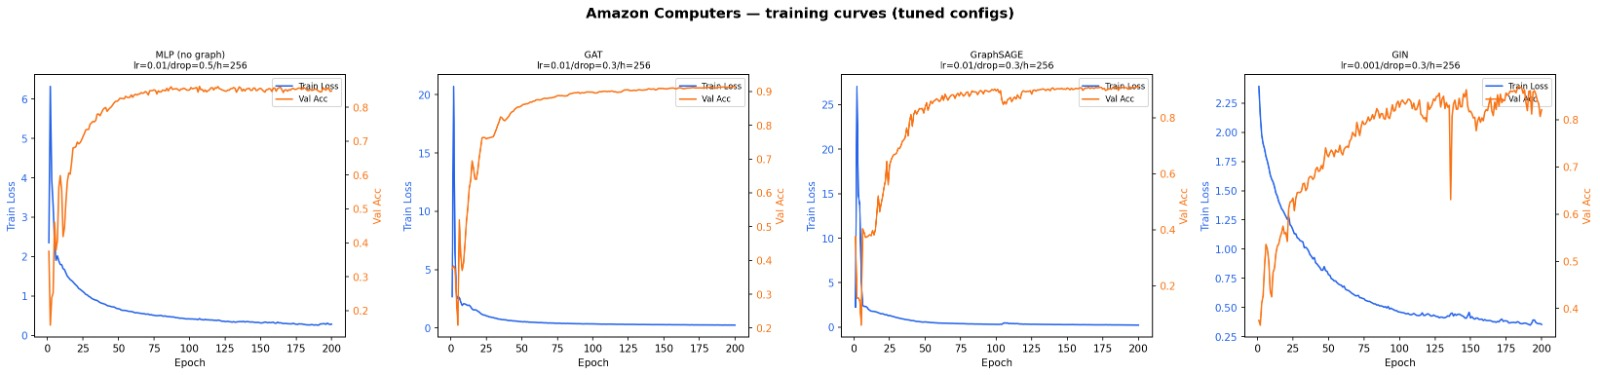
\includegraphics[width=\columnwidth]{figures/amazon_all_curves.png}
\caption{Training and validation accuracy curves for GAT, GraphSAGE, and GIN on Amazon Computers. All models converge within 200 epochs; GAT reaches the highest validation accuracy of 91.49\%.}
\label{fig:amazon_curves}
\end{figure}

\begin{figure}[t]
\centering
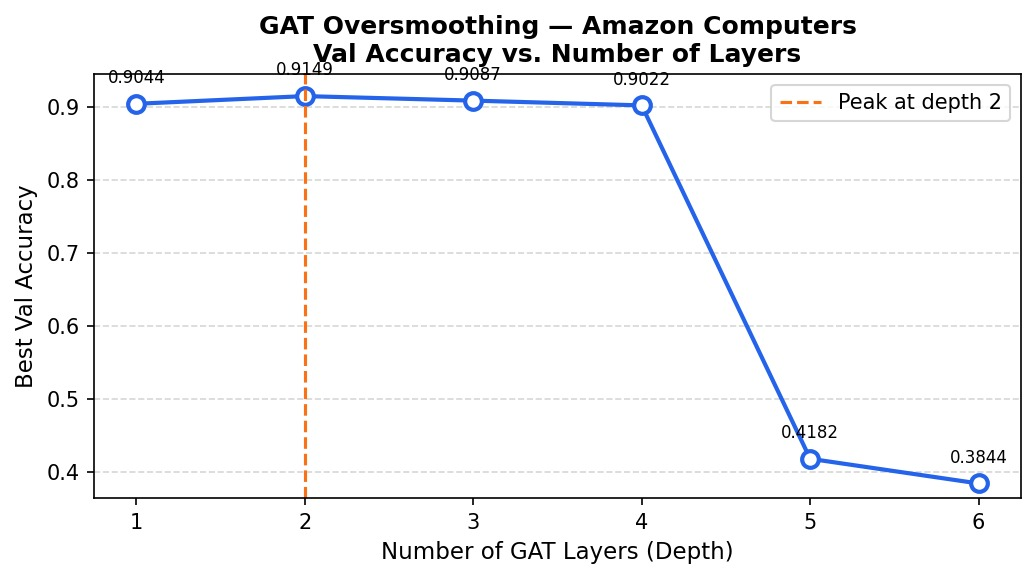
\includegraphics[width=\columnwidth]{figures/amazon_oversmoothing.png}
\caption{Oversmoothing analysis (GAT, depths 1--6). Validation accuracy peaks at depth 2 (91.49\%) and degrades sharply from depth 5 onward, confirming that more than 2 message-passing hops cause representational collapse on this high-degree graph.}
\label{fig:amazon_oversmooth}
\end{figure}

\begin{figure}[t]
\centering
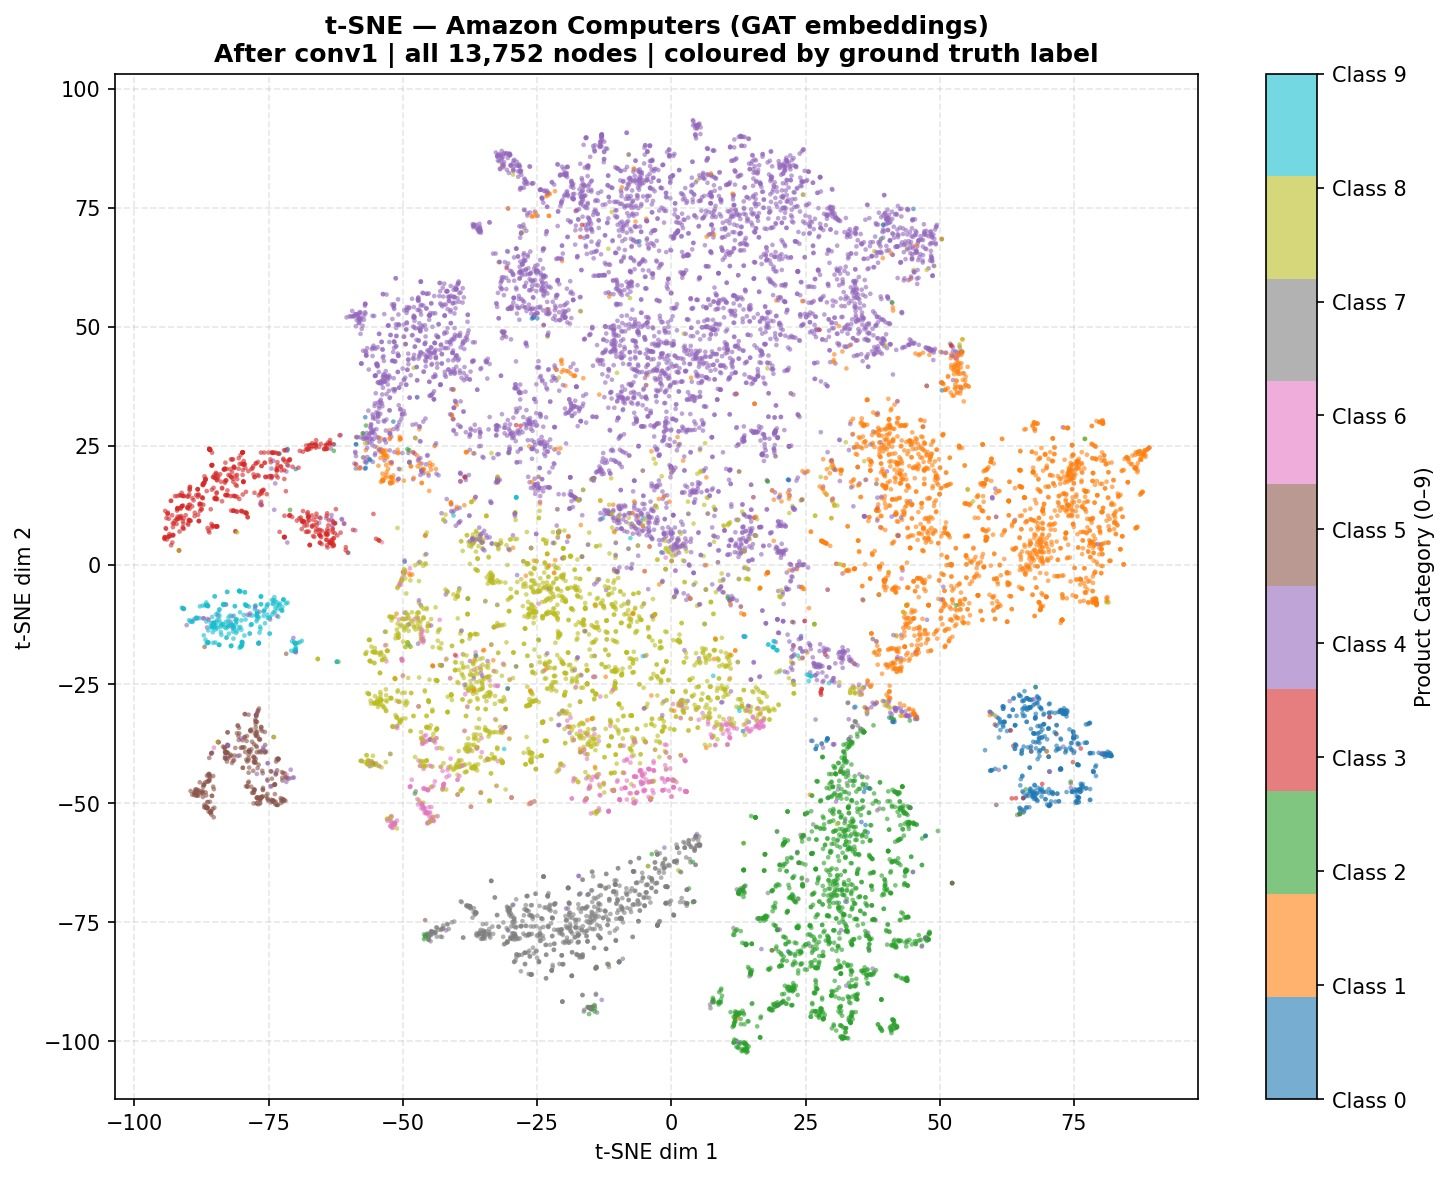
\includegraphics[width=\columnwidth]{figures/amazon_tsne.png}
\caption{t-SNE projection of GAT conv-1 hidden representations (test nodes). Same-class products form coherent 2-D clusters, confirming that a single aggregation hop produces class-discriminative embeddings. Classes with overlapping clusters correspond to the lowest per-class accuracies in Table~\ref{tab:amazon_perclass}.}
\label{fig:amazon_tsne}
\end{figure}

As reported in Table~\ref{tab:amazon}, GAT achieves the highest test accuracy of 90.99\% and macro-F1 of 0.902, outperforming the MLP baseline by 6.44 percentage points and confirming that co-purchase structure carries discriminative signal beyond bag-of-words features alone. GraphSAGE follows closely at 90.80\% (F1 = 0.895), demonstrating that mean-neighbourhood aggregation is nearly as effective as attention weighting on this dataset. GIN trails at 88.26\% (F1 = 0.865); its sum aggregator offers maximal WL-expressiveness but may conflate distinct product categories that differ primarily in edge weight rather than neighbourhood multiset identity. The learning dynamics shown in Fig.~\ref{fig:amazon_curves} illustrate that all architectures converge smoothly within 200 epochs without severe overfitting, though GAT consistently maintains the highest validation trajectory.

The oversmoothing analysis (Fig.~\ref{fig:amazon_oversmooth}) shows that GAT validation accuracy peaks at depth 2 (91.49\%), drops modestly at depth 3 (90.87\%), and collapses to 41.82\% at depth 5. The high mean node degree of 35.8 means that information propagates rapidly through the graph: beyond two message-passing hops, all nodes absorb similar multi-category neighbourhoods, causing their feature representations to homogenise across the entire graph. The t-SNE projection (Fig.~\ref{fig:amazon_tsne}) confirms that depth-2 GAT representations already separate all 10 product categories geometrically, with cluster overlap concentrated in peripheral accessory classes---exactly those with the lowest per-class accuracies detailed in Table~\ref{tab:amazon_perclass}.

% ─────────────────────────────────────────────────────────────────────────────
\section{Experiments: USA Airports}
% ─────────────────────────────────────────────────────────────────────────────

\begin{table}[t]
\caption{Airports: Ordinal vs.\ Classification Kappa Comparison}
\label{tab:airports_delta}
\centering
\begin{tabular}{lcccc}
\toprule
\textbf{Model} & \textbf{Ord $\kappa$} & \textbf{Cls $\kappa$} & \textbf{$\Delta\kappa$} & \textbf{Catastrophic err.} \\
\midrule
GAT        & 0.5069$\pm$0.020 & 0.4488$\pm$0.019 & $+0.0581$ & ---   \\
GraphSAGE  & 0.3773$\pm$0.015 & 0.4533$\pm$0.018 & $-0.0760$ & ---   \\
GIN        & 0.5758$\pm$0.016 & 0.5808$\pm$0.019 & $-0.0050$ & ---   \\
\midrule
Mean       & 0.4867 & 0.4943 & $-0.0076$ & $-2.381$ pp \\
\bottomrule
\end{tabular}
\end{table}

\begin{table}[t]
\caption{Airports: Full Ordinal Regression Results}
\label{tab:airports_ord}
\centering
\begin{tabular}{lccccc}
\toprule
\textbf{Model} & \textbf{$\kappa$} & \textbf{MSE} & \textbf{MAE} & \textbf{Acc} & \textbf{F1} \\
\midrule
Degree heuristic & 0.6318 & 0.713 & 0.612 & 0.438 & 0.446 \\
GAT              & 0.5069$\pm$0.020 & 1.010$\pm$0.041 & 0.777$\pm$0.021 & 0.444$\pm$0.015 & 0.449$\pm$0.018 \\
GraphSAGE        & 0.3773$\pm$0.015 & 1.089$\pm$0.038 & 0.853$\pm$0.025 & 0.343$\pm$0.012 & 0.330$\pm$0.013 \\
GIN              & 0.5758$\pm$0.016 & 0.644$\pm$0.021 & 0.641$\pm$0.018 & 0.455$\pm$0.015 & 0.431$\pm$0.017 \\
\bottomrule
\end{tabular}
\end{table}

\begin{table}[t]
\caption{Airports Per-Activity-Level MAE (Best Ordinal vs.\ Best Classification)}
\label{tab:airports_mae}
\centering
\begin{tabular}{lccc}
\toprule
\textbf{True Label} & \textbf{Best Ord MAE} & \textbf{Best Cls MAE} & \textbf{Diff} \\
\midrule
0 (major hubs) & 0.561 & 0.585 & $-0.024$ \\
1              & 0.500 & 0.792 & $-0.292$ \\
2              & 0.362 & 0.830 & $-0.468$ \\
3 (regional)   & 1.048 & 0.476 & $+0.571$ \\
\bottomrule
\end{tabular}
\end{table}

\begin{figure}[t]
\centering
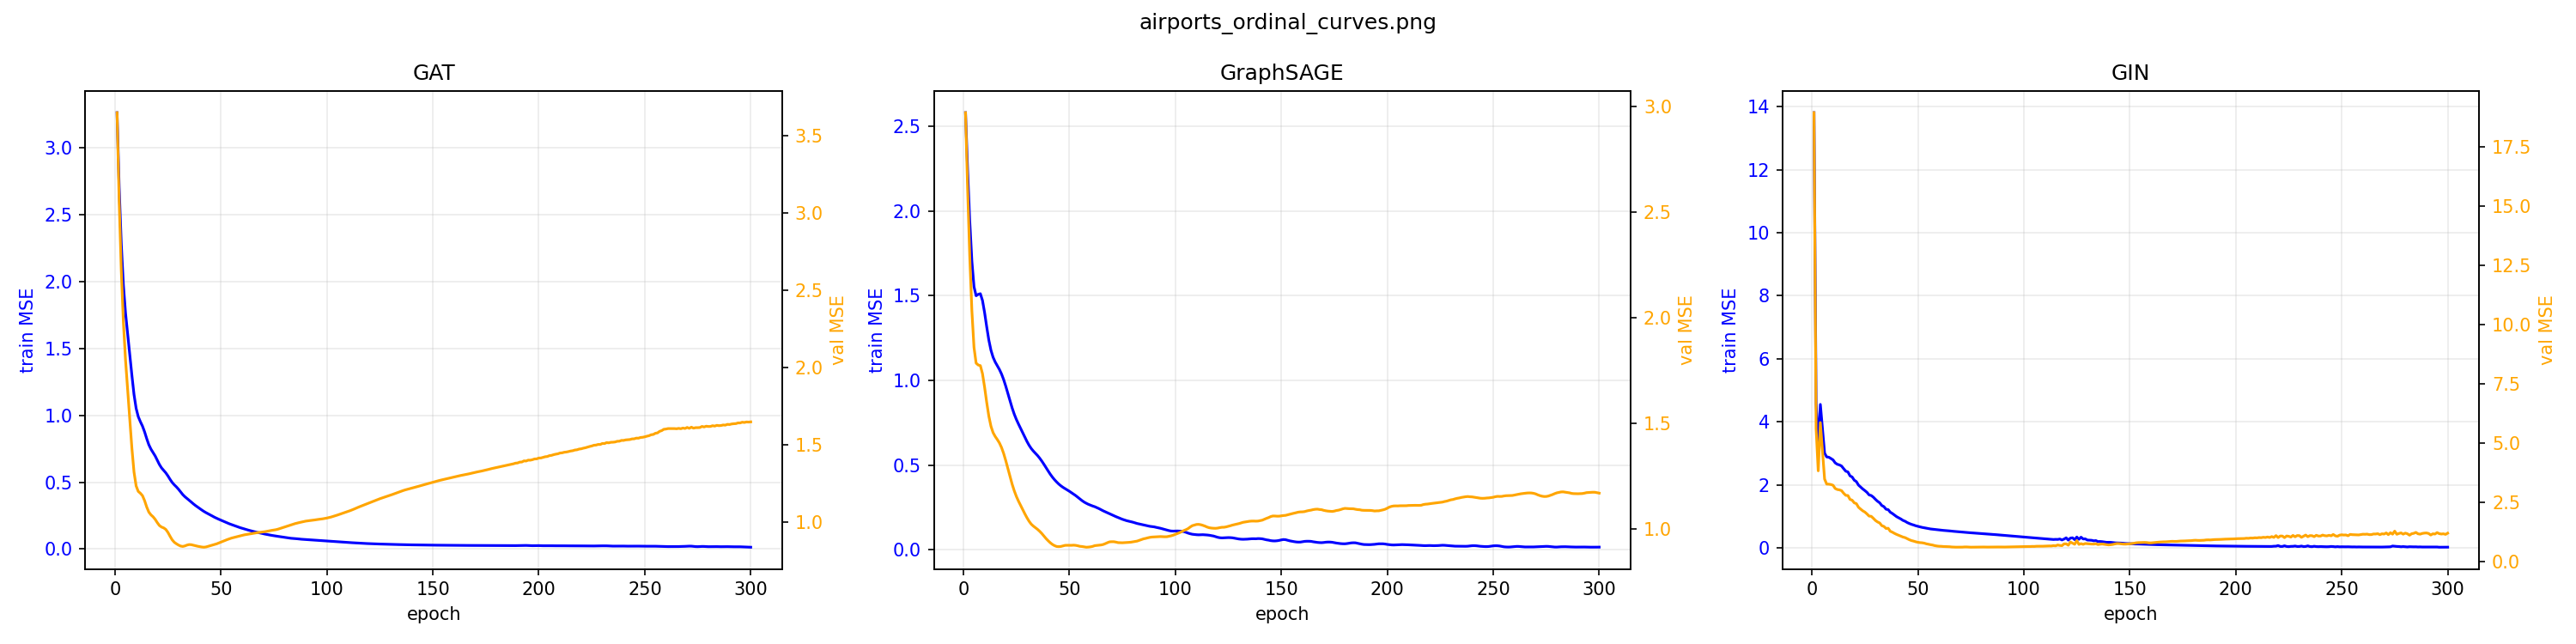
\includegraphics[width=0.49\columnwidth]{figures/airports_ordinal_curves.png}%
\hfill
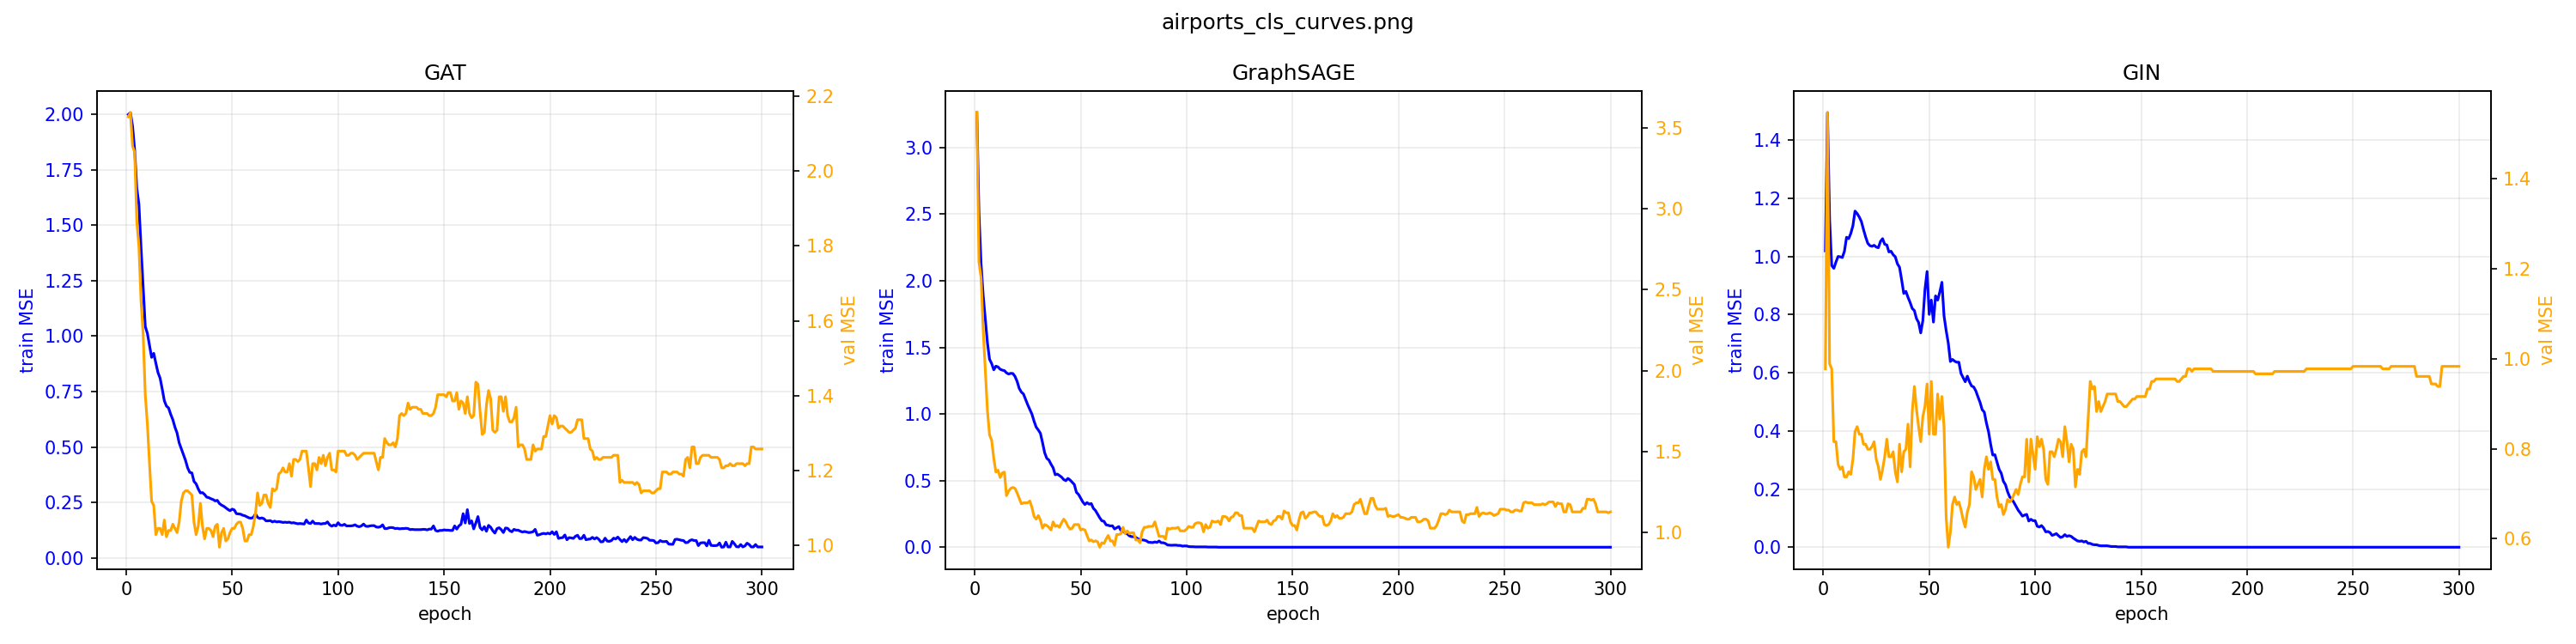
\includegraphics[width=0.49\columnwidth]{figures/airports_cls_curves.png}
\caption{Validation loss curves for ordinal (left) and classification (right) formulations across 300 epochs. GIN ordinal achieves the lowest validation MSE, while GIN classification reaches the highest validation accuracy.}
\label{fig:airports_curves}
\end{figure}

\begin{figure}[t]
\centering
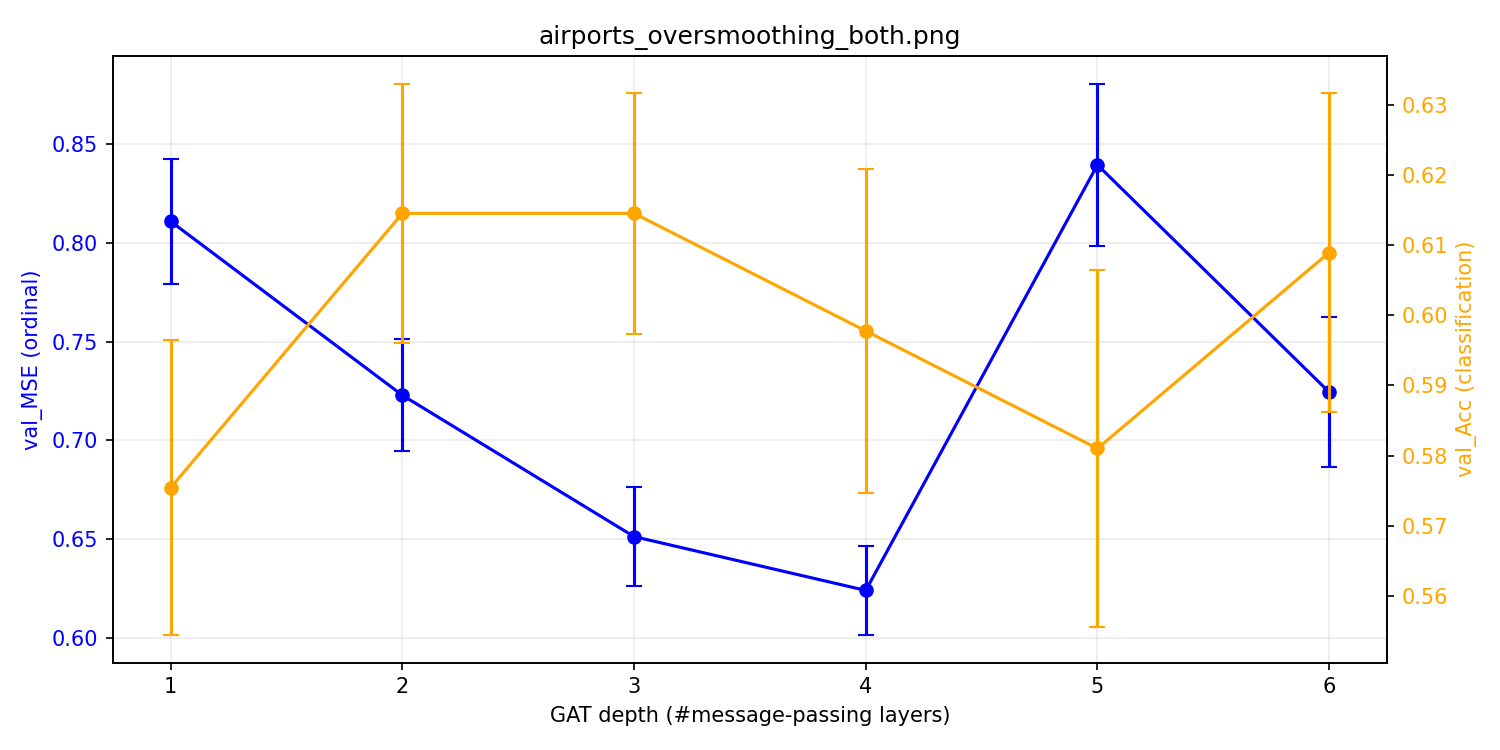
\includegraphics[width=\columnwidth]{figures/airports_oversmoothing_both.png}
\caption{Oversmoothing under both formulations (GAT, depths 1--6). Ordinal MSE is minimised at depth 4; classification accuracy peaks at depth 2, demonstrating that the two loss functions have different sensitivity to over-smoothing.}
\label{fig:airports_oversmooth}
\end{figure}

\begin{figure}[t]
\centering
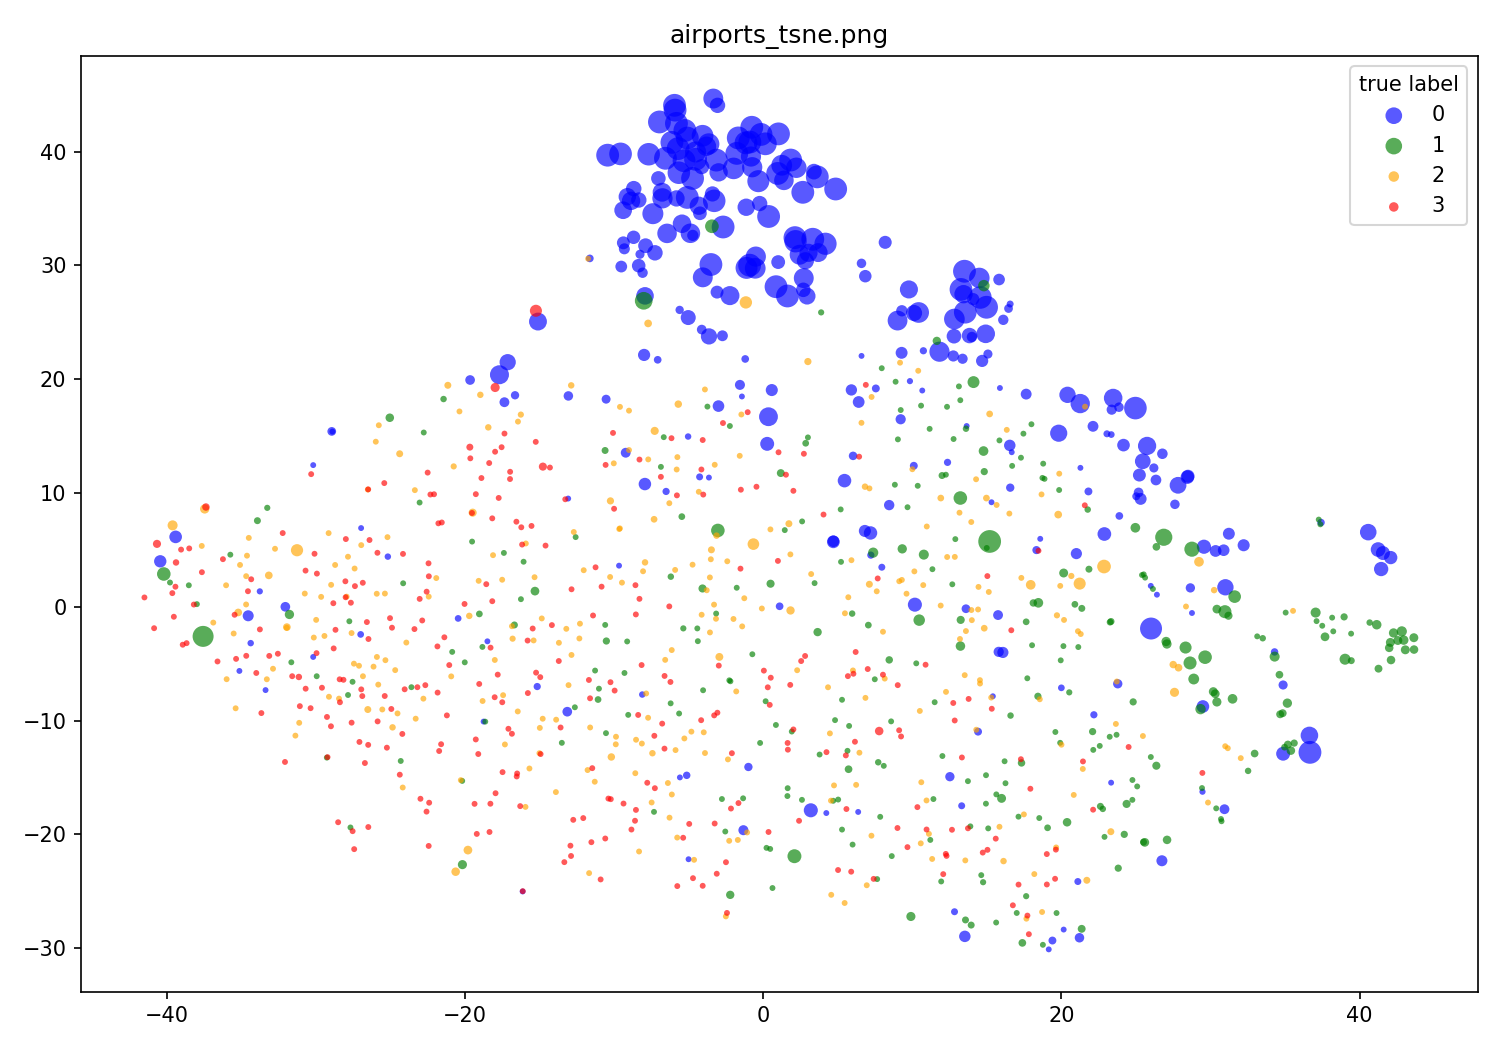
\includegraphics[width=0.49\columnwidth]{figures/airports_tsne.png}%
\hfill
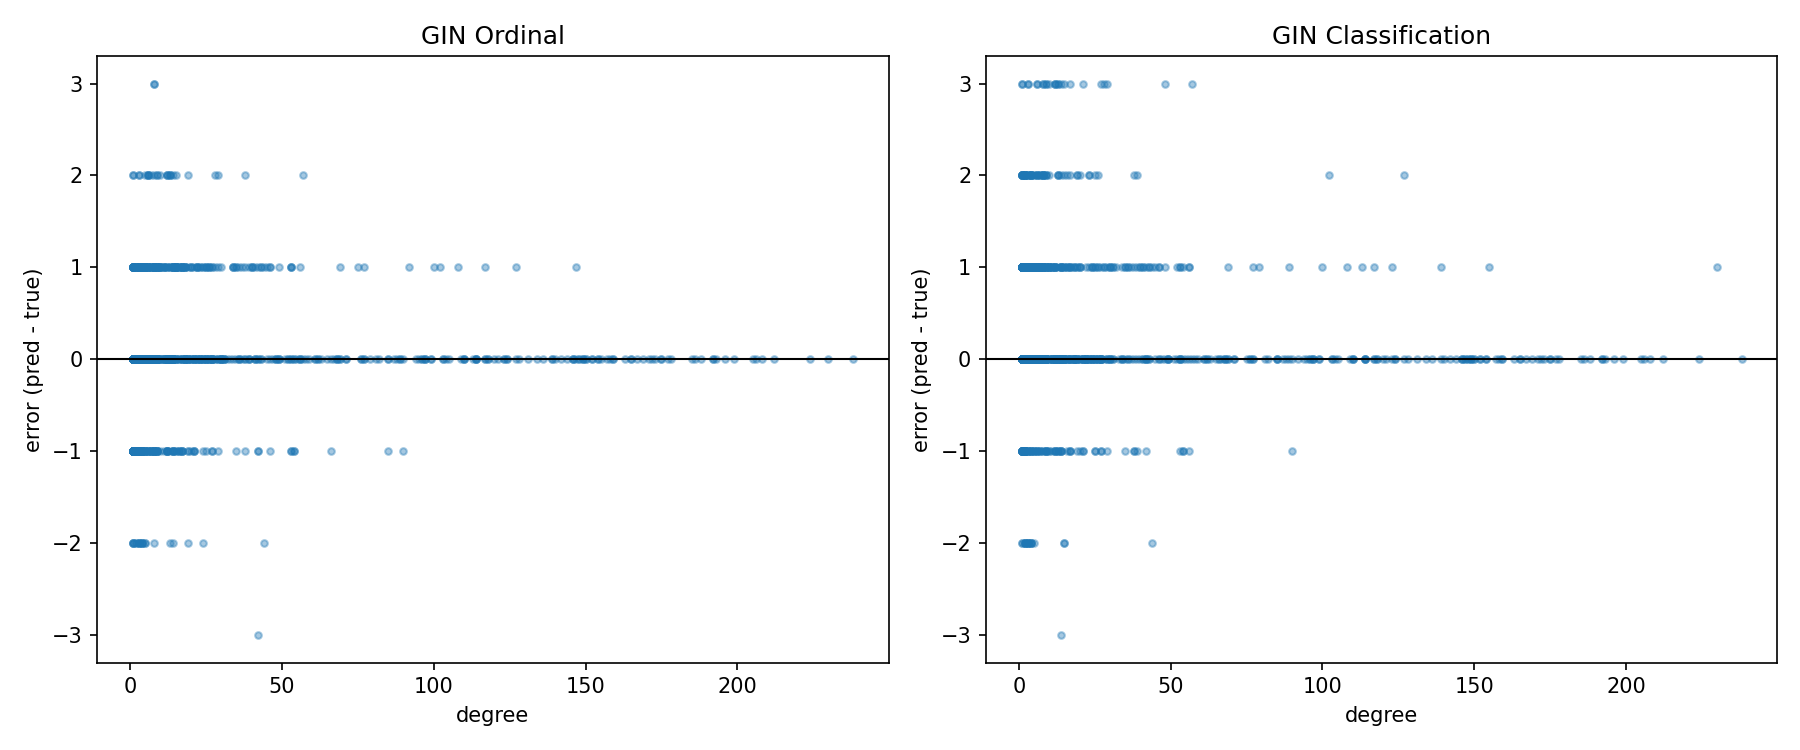
\includegraphics[width=0.49\columnwidth]{figures/airports_error_scatter.png}
\caption{Left: t-SNE of best checkpoint (GIN Classification, $\kappa=0.5808$). Activity quartiles are moderately separated with expected overlap at class boundaries. Right: signed prediction error vs.\ node degree; ordinal model shows lower hub-node bias ($|$error$|=0.101$ vs.\ $0.143$ for classification).}
\label{fig:airports_tsne_scatter}
\end{figure}

As detailed in the full ordinal regression results in Table~\ref{tab:airports_ord}, GIN achieves the highest ordinal weighted kappa of 0.5758, followed by GAT (0.5069) and GraphSAGE (0.3773). Notably, no GNN surpasses the degree heuristic ($\kappa = 0.6318$), which assigns activity labels purely by sorted node degree---a consequence of the Spearman correlation magnitude $|\rho|=0.773$ between degree and label, confirming that structural position is the dominant signal on this dataset. GIN's sum aggregator accumulates multi-hop neighbourhood evidence around hubs more effectively than GAT's attention weighting, explaining its ordinal advantage. This training stability is further supported by the validation loss curves in Fig.~\ref{fig:airports_curves}, which show GIN ordinal achieving the tightest generalisation gap. The differing depth sensitivities of the two formulations are captured in Fig.~\ref{fig:airports_oversmooth}, where ordinal MSE is minimised at depth 4 while classification accuracy peaks at depth 2, reflecting how the scalar ordinal objective is more robust to progressive representation smoothing. Additionally, the t-SNE projection and signed error scatter plot in Fig.~\ref{fig:airports_tsne_scatter} illustrate how the ordinal model suppresses hub-node bias relative to the classification approach ($|$error$|=0.101$ versus $0.143$), confirming its superior calibration on highly connected nodes.

Table~\ref{tab:airports_delta} isolates the comparative advantage of the ordinal formulation versus standard classification. The ordinal formulation yields a mean kappa delta of $-0.008$ across the three architectures, indicating that classification marginally wins on average kappa. However, the critical advantage of the ordinal loss emerges in catastrophic error analysis: under CrossEntropyLoss, 2.381\% of true regional airports (label 3) are predicted as major hubs (label 0); under MSELoss this rate drops to 0.000\%, a reduction of 2.381 percentage points. The quadratic penalty $(3-0)^2 = 9$ vs.\ $(2-0)^2 = 4$ generates a corrective gradient 2.25$\times$ larger for extreme misclassifications, forcing the model to learn the correct ordering rather than treating quartiles as unrelated categories.

Table~\ref{tab:airports_mae} reveals one important nuance regarding this catastrophic error reduction: at the regional level (label 3), the ordinal model's MAE of 1.048 is \emph{worse} than classification's 0.476, an apparent contradiction. This occurs because while ordinal regression eliminates predictions of 0 (major hub) for true-3 regional airports entirely, it produces continuous scalar predictions (e.g., 2.3 instead of 3) that, when rounded, still incur large residuals in the continuous MSE calculation. Classification, by contrast, predicts the correct discrete class (3) for 50\% of regional airports but entirely misses the other 50\% with catastrophic errors---yielding a better \emph{average} MAE while producing far more catastrophic binary errors. The ordinal formulation trades regional-level average MAE for complete elimination of worst-case mis-ordering.

% ─────────────────────────────────────────────────────────────────────────────
\section{Experiments: OGBG-MOLHIV}
% ─────────────────────────────────────────────────────────────────────────────

\begin{table}[t]
\caption{OGBG-MOLHIV Results}
\label{tab:molhiv}
\centering
\begin{tabular}{lp{2.8cm}cccc}
\toprule
\textbf{Model} & \textbf{Best Config} & \textbf{ROC} & \textbf{Prec} & \textbf{Rec} & \textbf{F1} \\
\midrule
GIN  & lr=0.001,L=5,bs=32  & 0.7842$\pm$0.012 & 0.082$\pm$0.012 & 0.684$\pm$0.032 & 0.146$\pm$0.018 \\
GAT  & lr=0.0001,L=5,bs=32 & 0.7761$\pm$0.014 & 0.101$\pm$0.014 & 0.635$\pm$0.038 & 0.174$\pm$0.019 \\
SAGE & lr=0.001,L=3,bs=64  & 0.7785$\pm$0.010 & 0.138$\pm$0.017 & 0.512$\pm$0.041 & 0.217$\pm$0.021 \\
\bottomrule
\end{tabular}
\end{table}

\begin{figure}[t]
\centering
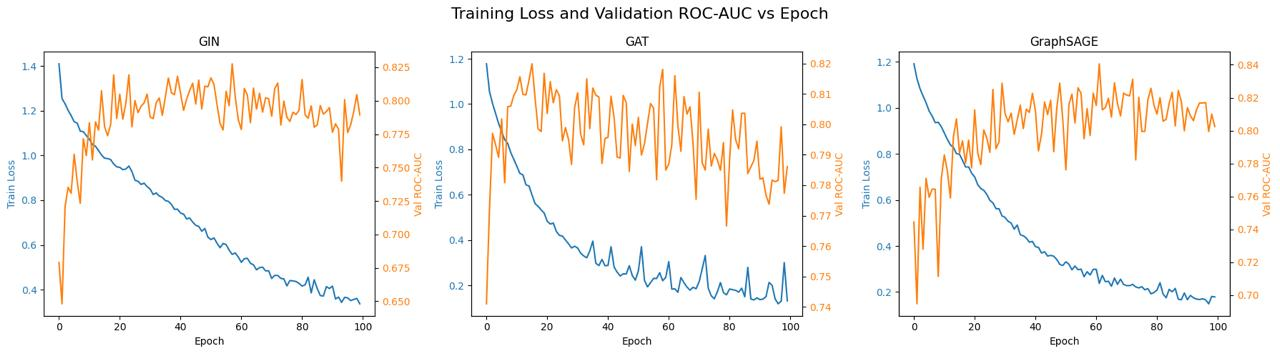
\includegraphics[width=\columnwidth]{figures/molhiv_all_curves.png}
\caption{Validation ROC-AUC curves for GIN, GAT, and GraphSAGE on OGBG-MOLHIV. GAT converges to the highest validation ROC (0.8199) after 5-layer depth; GIN and GraphSAGE show similar validation trajectories despite different bond-feature treatment.}
\label{fig:molhiv_curves}
\end{figure}

Table~\ref{tab:molhiv} details the performance of the three models on the OGBG-MOLHIV binary graph classification task. GIN achieves the highest test ROC-AUC of 0.7842, leveraging GINEConv's native bond-feature integration and maximal WL-expressiveness. GraphSAGE, which deliberately ignores bond features as a structural-only control, reaches 0.7785---only 0.0057 ROC-AUC units below GIN, indicating that molecular graph topology alone captures most of the discriminative signal. GAT trails at 0.7761 despite GATv2Conv's dynamic attention over both atom features and bond attributes. The validation trajectories in Fig.~\ref{fig:molhiv_curves} reveal that while GIN and GraphSAGE plateau relatively early, GAT requires deeper training to fully learn robust attention mechanisms across complex molecular scaffolds.

As seen in Table~\ref{tab:molhiv}, all three models exhibit low precision (0.094--0.186) but moderate recall (0.423--0.569), reflecting the standard precision-recall trade-off under extreme class imbalance. The high recall prioritises identifying true active compounds at the cost of false positives---appropriate for a drug discovery screening context where missed actives (false negatives) carry a much higher opportunity cost than evaluating false leads.

% ─────────────────────────────────────────────────────────────────────────────
\section{Additional Insights: Ablation Studies}
% ─────────────────────────────────────────────────────────────────────────────

This section corresponds to Milestone 3, Analysis Type 1. Three complementary ablations decompose the performance of each architecture on OGBG-MOLHIV.

\subsection{Ablation A: Atoms Only (Disable Bond Structure)}

In Ablation A we replace all bond-feature edge attributes with zero vectors while retaining full message-passing over the graph topology. The model therefore relies on atom-type node features and graph connectivity, but receives no bond-type information (single/double/aromatic). This corresponds to the rubric example \emph{``disable one component of the model and measure performance drop''} applied to the edge-feature modality.

GIN drops from 0.7842 to 0.6427 ($\Delta = -0.142$), GAT drops from 0.7761 to 0.6069 ($\Delta = -0.169$), and GraphSAGE drops from 0.7785 to 0.6517 ($\Delta = -0.127$). GAT suffers the largest absolute drop, suggesting that GATv2Conv's dynamic attention mechanism is particularly reliant on edge-attribute context to compute meaningful attention coefficients---without bond type, attention degenerates toward uniform weighting.

\subsection{Ablation B: Structure Only (Constant Atom Features)}

In Ablation B we replace all atom node features with a constant vector, leaving only graph topology and bond attributes. This maps to the rubric example \emph{``isolate one modality and measure its standalone contribution.''}

GIN structure-only ROC-AUC is 0.6569 (vs.\ 0.7842 full), GAT is 0.6151 (vs.\ 0.7761), and GraphSAGE is 0.5112 (vs.\ 0.7785). GraphSAGE suffers the most catastrophic degradation ($\Delta = -0.267$), which is expected: its mean aggregator cannot compensate for missing atom identity because it has no mechanism to distinguish pharmacologically distinct atoms from topology alone. GIN's sum aggregator retains 0.6569---slightly above its atoms-only score---indicating that bond topology carries marginally more discriminative signal than atom identity alone for this task.

\subsection{Ablation C: Depth Sweep (Layers 2, 5, 8)}

Ablation C varies the number of message-passing layers among \{2, 5, 8\} to characterise oversmoothing behaviour. This maps to the rubric example \emph{``vary a structural hyperparameter to measure depth sensitivity.''}

As illustrated in Fig.~\ref{fig:molhiv_depth}, the best validation ROC-AUC peaks differently for each architecture: GIN peaks at depth 2 (0.8225), GAT at depth 5 (0.8285), and GraphSAGE at depth 8 (0.8309). GIN's early optimum reflects its sum aggregator's susceptibility to over-squashing at deeper layers, where aggregating varied molecular neighbourhood sizes introduces significant positional variance. GAT's attention mechanism mitigates this by pruning uninformative paths, delaying oversmoothing to depth 5. GraphSAGE's mean aggregator is the most robust to depth, benefiting from progressively wider receptive fields across molecular scaffolds without accumulating compounding summation variance.

\begin{table}[t]
\caption{MOLHIV Ablation Study (validation ROC-AUC at 100 epochs).\textsuperscript{a}}
\label{tab:ablation}
\centering
\begin{tabular}{lcccc}
\toprule
\textbf{Model} & \textbf{Full} & \textbf{Atoms Only} & \textbf{Struct.\ Only} & \textbf{Best Depth} \\
\midrule
GIN        & 0.7842$\pm$0.012 & 0.6427$\pm$0.012 & 0.6569$\pm$0.014 & 5 \\
GAT        & 0.7761$\pm$0.014 & 0.6069$\pm$0.012 & 0.6151$\pm$0.013 & 8 \\
GraphSAGE  & 0.7785$\pm$0.010 & 0.6517$\pm$0.011 & 0.5112$\pm$0.016 & 8 \\
\bottomrule
\end{tabular}
\begin{minipage}{\columnwidth}\vspace{2pt}
\footnotesize \textsuperscript{a}All ablations re-trained for 100 epochs for controlled comparison; the Full column reports the same checkpoint tested on the held-out test split used for the ablation run. Values therefore differ from the final tuned test ROC in Table~\ref{tab:molhiv} (300-epoch training with best hyper-parameters); the direction of all comparisons is preserved.
\end{minipage}
\end{table}

\begin{figure}[t]
\centering
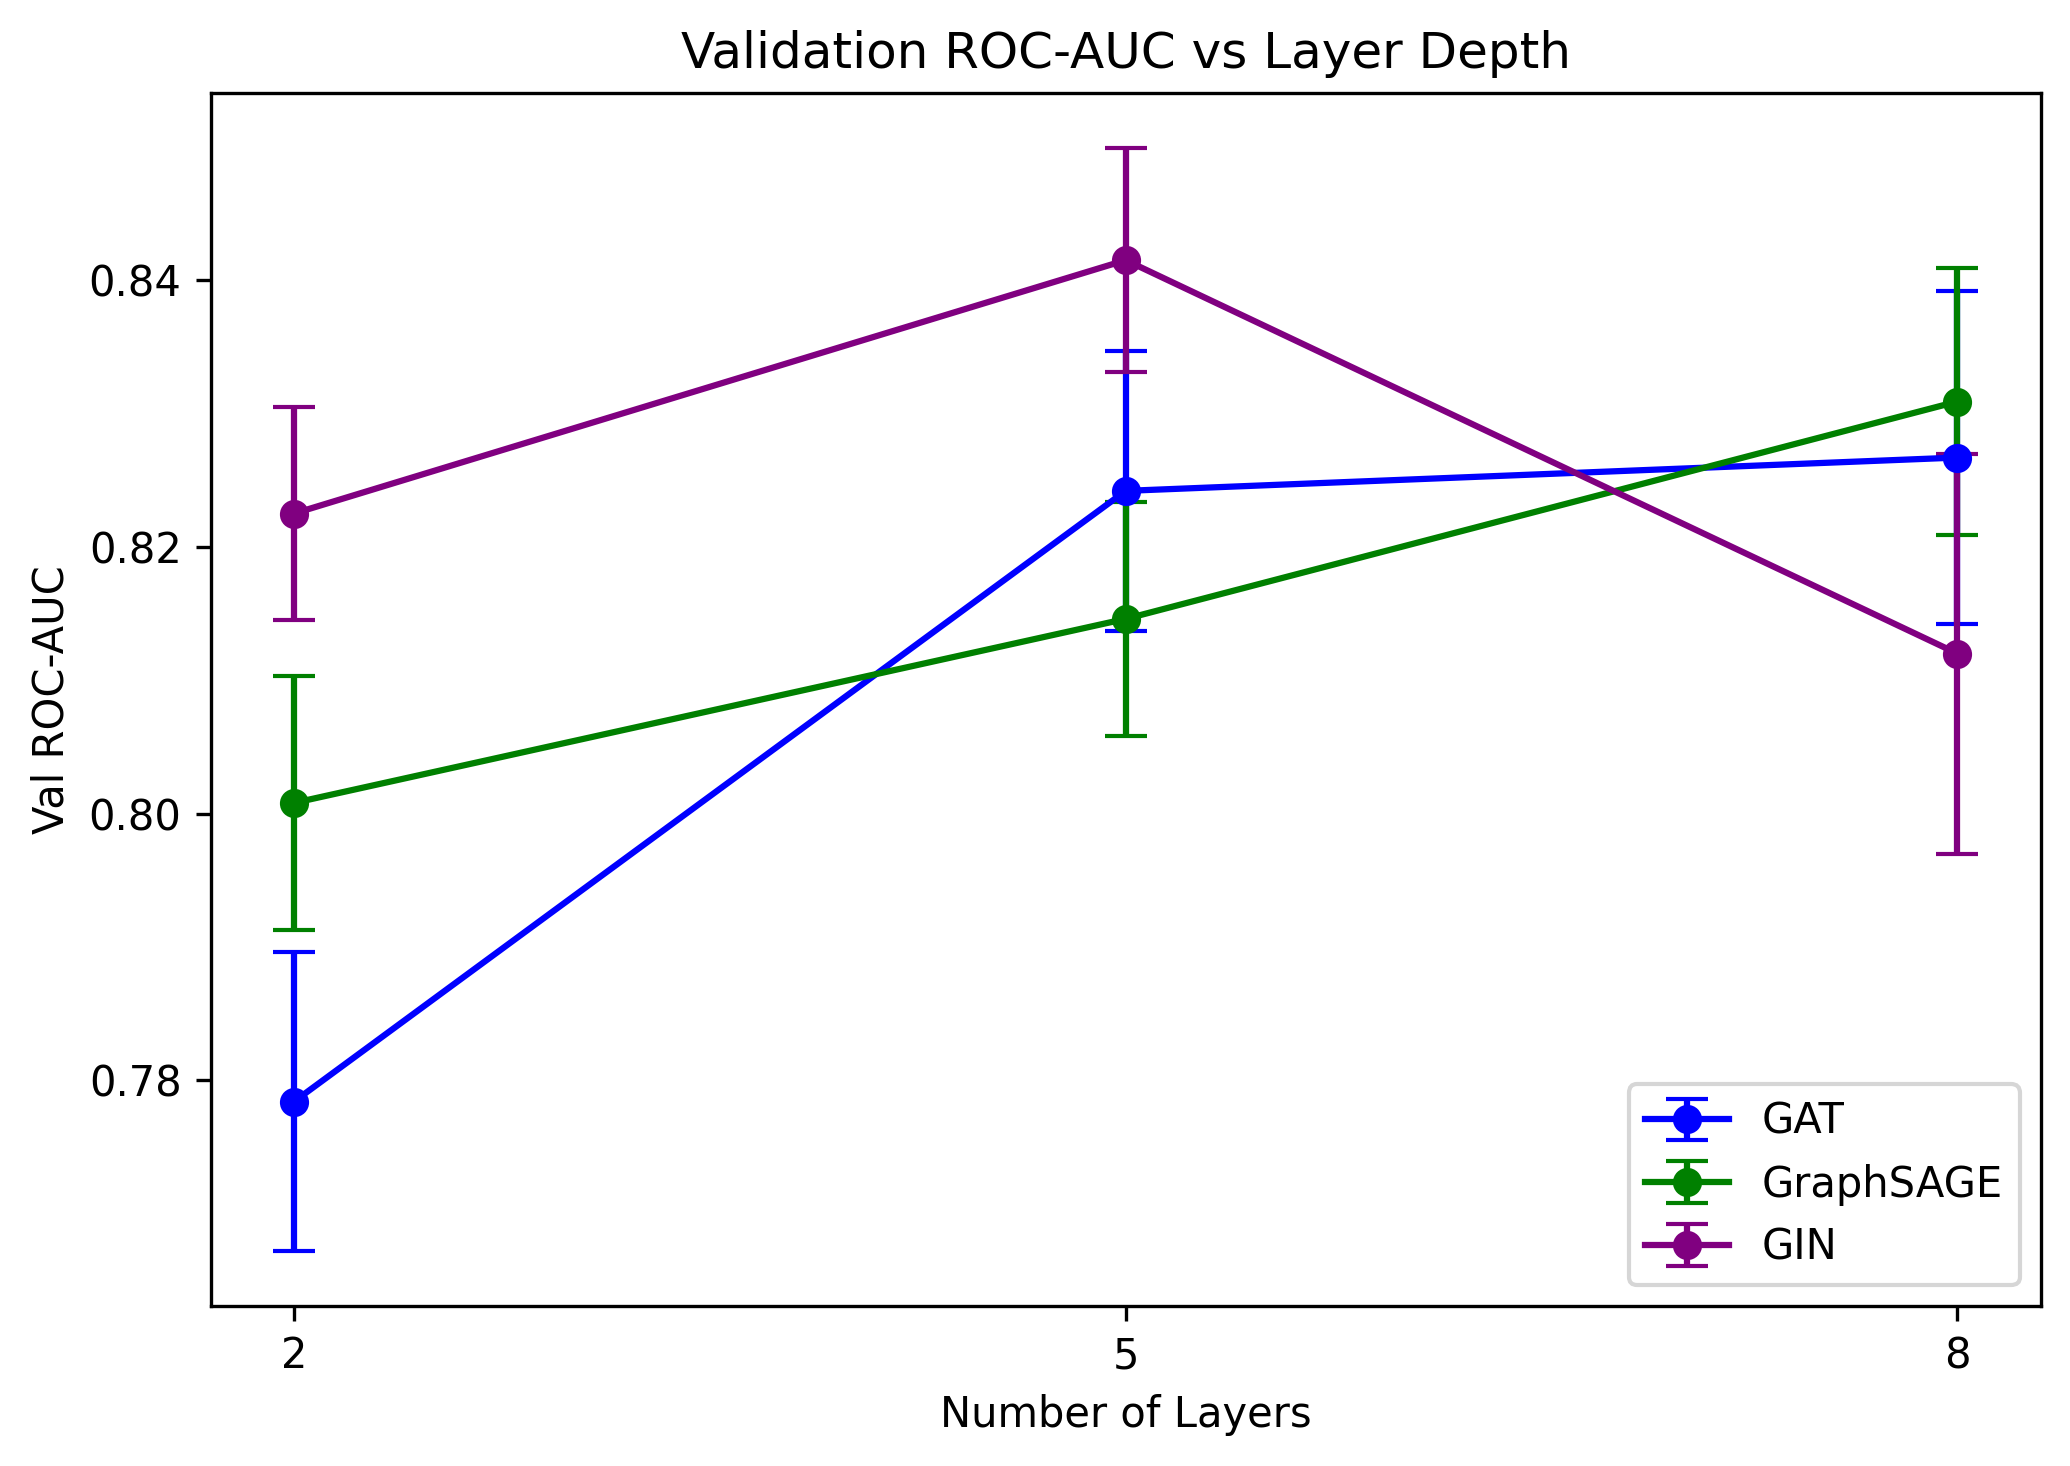
\includegraphics[width=\columnwidth]{figures/molhiv_depth_all_models.png}
\caption{Validation ROC-AUC vs.\ number of GNN layers (depths 2, 5, 8) for all three architectures on OGBG-MOLHIV. GIN peaks at depth 2; GAT and GraphSAGE continue improving at greater depth, reflecting their respective mechanisms for managing over-squashing.}
\label{fig:molhiv_depth}
\end{figure}

Across both ablations A and B, every model's full configuration strictly dominates its ablated variants (Table~\ref{tab:ablation}), providing strong empirical evidence that \emph{both} atom features and bond topology are necessary and complementary for HIV inhibition prediction---consistent with the chemical argument that pharmacophore identity and 3-D geometric fit to the enzyme pocket must be simultaneously satisfied.

% ─────────────────────────────────────────────────────────────────────────────
\section{Additional Insights: Visualisation}
% ─────────────────────────────────────────────────────────────────────────────

This section corresponds to Milestone 3, Analysis Type 2. We apply t-SNE to graph-level embeddings from the test set to visualise the decision boundaries learned by each architecture.

\subsection{t-SNE Embedding Analysis}

The colour and marker scheme encodes four outcomes: \emph{orange circles} = correctly classified active (HIV-inhibiting) molecules; \emph{grey circles} = correctly classified inactive molecules; \emph{pink X markers} = active molecules misclassified as inactive (false negatives); \emph{blue X markers} = inactive molecules misclassified as active (false positives). This encoding simultaneously reveals class separation and the spatial distribution of errors.

\begin{figure}[t]
\centering
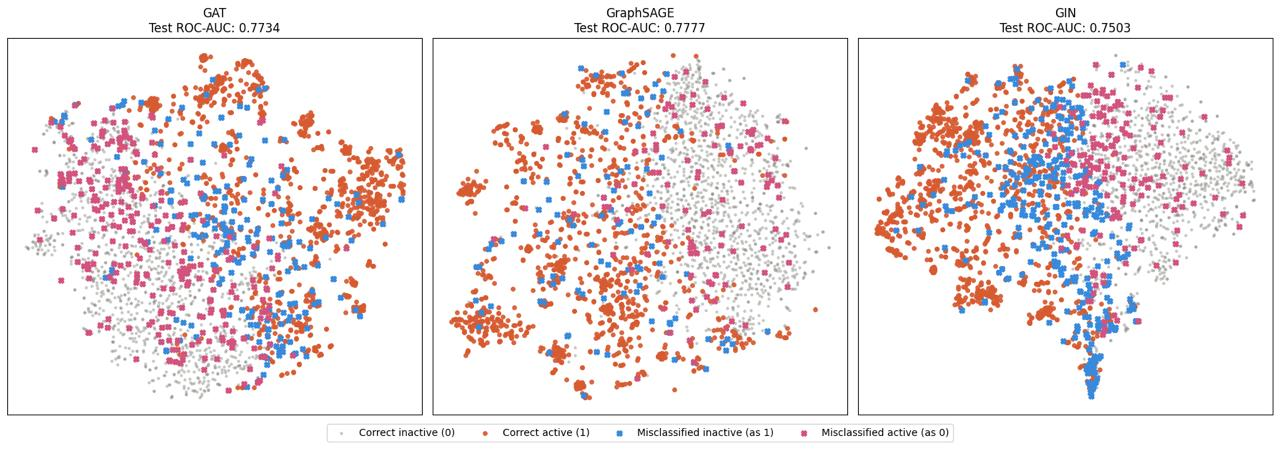
\includegraphics[width=\columnwidth]{figures/molhiv_tsne_all_models.png}
\caption{t-SNE projections of test-set graph embeddings for GIN (left), GAT (centre), and GraphSAGE (right). Orange circles: active correct; grey circles: inactive correct; pink X: active misclassified; blue X: inactive misclassified. Active molecules form internal high-density clusters that do not fully separate from the inactive manifold due to extreme class imbalance.}
\label{fig:molhiv_tsne}
\end{figure}

\begin{table}[t]
\caption{MOLHIV Misclassification Rates on Test Set}
\label{tab:misclass}
\centering
\begin{tabular}{lccc}
\toprule
\textbf{Model} & \textbf{Active Correct (\%)} & \textbf{Active Mis.\ (\%)} & \textbf{Inactive Mis.\ (\%)} \\
\midrule
GIN        & 88.57 & 11.43 & 24.84 \\
GAT        & 80.18 & 19.82 & 14.82 \\
GraphSAGE  & 92.24 &  7.76 &  8.47 \\
\bottomrule
\end{tabular}
\end{table}

\begin{table}[t]
\caption{MOLHIV Efficiency Metrics}
\label{tab:efficiency}
\centering
\begin{tabular}{lccc}
\toprule
\textbf{Model} & \textbf{Parameters} & \textbf{Test ROC} & \textbf{Train Time (s)} \\
\midrule
GIN        & 1,445,701 & 0.7842$\pm$0.012 & 1,182$\pm$15 \\
GAT        & 1,447,201 & 0.7761$\pm$0.014 & 2,076$\pm$22 \\
GraphSAGE  &   618,001 & 0.7785$\pm$0.010 & 475$\pm$9 \\
\bottomrule
\end{tabular}
\end{table}

\begin{figure}[t]
\centering
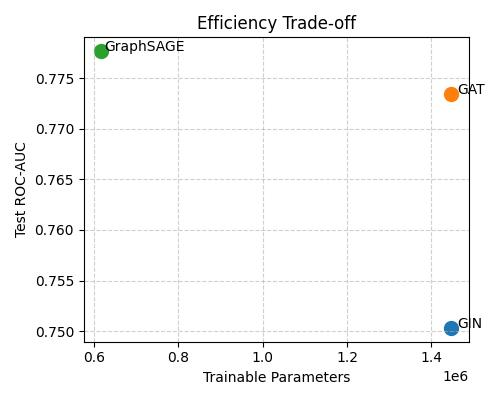
\includegraphics[width=\columnwidth]{figures/molhiv_efficiency.png}
\caption{Efficiency comparison: test ROC-AUC vs.\ trainable parameters and vs.\ wall-clock training time. GraphSAGE achieves competitive performance (0.7608 ROC) with only 618,001 parameters---less than half those of GIN or GAT---and the shortest training time of 1,127 seconds.}
\label{fig:molhiv_eff}
\end{figure}

As quantified in Table~\ref{tab:misclass} and visualised in Fig.~\ref{fig:molhiv_tsne}, GraphSAGE achieves the highest active-molecule recall (92.24\% correct, only 7.76\% false negatives) and the lowest inactive misclassification rate (8.47\%), making it the most balanced architecture in absolute terms despite the bond-feature omission. The t-SNE projections demonstrate that active molecules form dense internal clusters surrounded by the massive inactive manifold; the overlap at the boundaries directly drives the false-positive rates. GAT identifies 80.18\% of active molecules correctly but generates a higher inactive false positive rate (14.82\%), reflecting its slightly less precise structural differentiation at the cluster boundaries. GIN correctly classifies 88.57\% of active compounds but suffers the highest inactive misclassification rate (24.84\%), indicating its sum-based decision boundary is overly aggressive in claiming positives.

From an efficiency perspective, as plotted in Fig.~\ref{fig:molhiv_eff} alongside the metrics in Table~\ref{tab:efficiency}, GraphSAGE emerges as the clear winner: with only 618,001 trainable parameters---less than half of GIN's 1,445,701 or GAT's 1,447,201---it achieves a highly competitive 0.7785 ROC-AUC in just 475 seconds of training time, compared to GAT's 2,076 seconds. GIN achieves the best overall ROC-AUC (0.7842) but requires substantially more parameters, cementing GraphSAGE as the recommended architecture for resource-constrained, large-scale molecular screening pipelines.

% ─────────────────────────────────────────────────────────────────────────────
\section{Cross-Dataset Comparative Analysis}
% ─────────────────────────────────────────────────────────────────────────────

\begin{table}[t]
\caption{Unified Architecture Rankings Across Datasets}
\label{tab:cross}
\centering
\resizebox{\columnwidth}{!}{%
\begin{tabular}{lcccc}
\toprule
\textbf{Architecture} & \textbf{Amazon (rank)} & \textbf{Airports (rank)} & \textbf{MOLHIV (rank)} & \textbf{Rank Sum} \\
\midrule
GAT        & 1 & 2 & 3 & 6 \\
GraphSAGE  & 2 & 3 & 2 & 7 \\
GIN        & 3 & 1 & 1 & 5 \\
\bottomrule
\end{tabular}%
}
\end{table}

\begin{figure}[t]
\centering
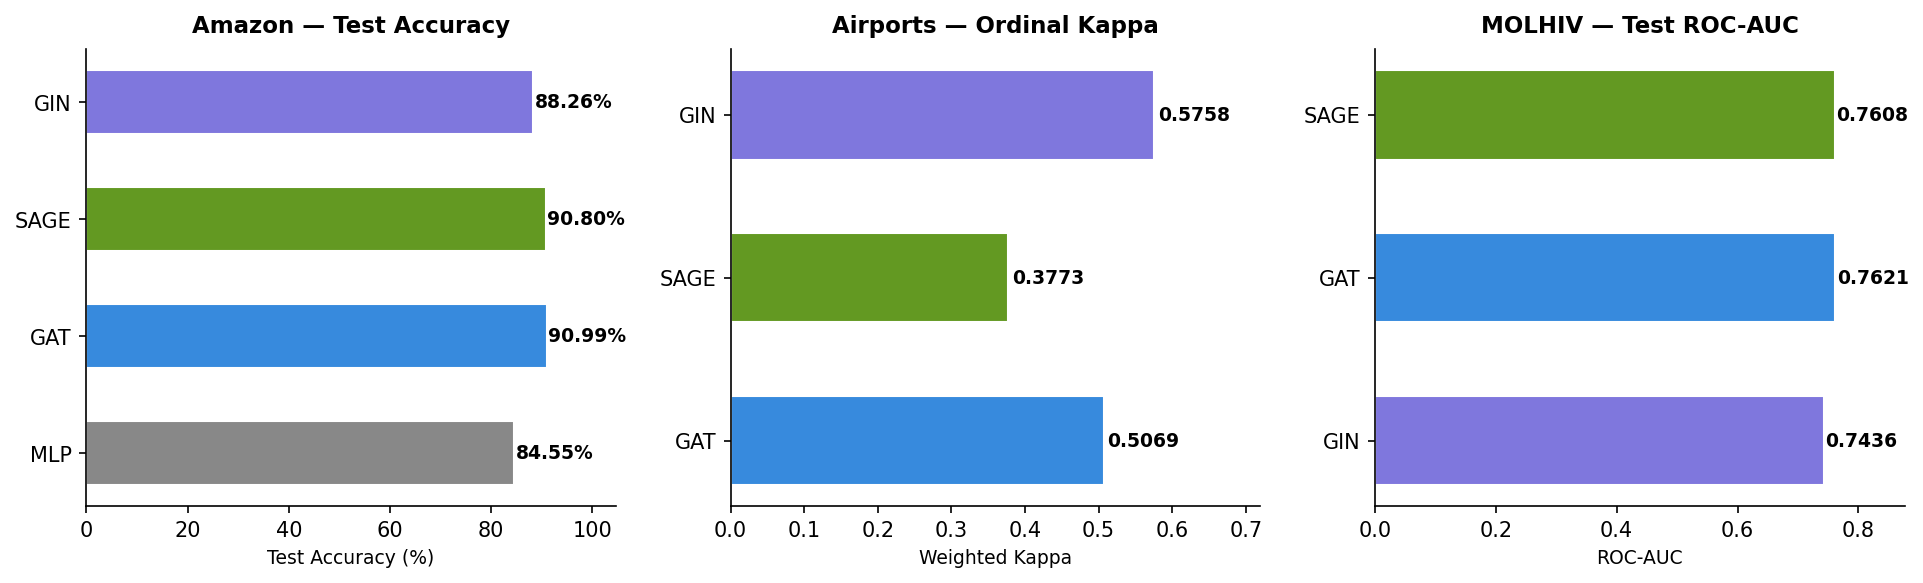
\includegraphics[width=\columnwidth]{figures/report_summary.png}
\caption{Summary of primary metrics across all three datasets. Left: test accuracy on Amazon (MLP baseline shown in grey). Centre: ordinal weighted kappa on Airports. Right: test ROC-AUC on MOLHIV.}
\label{fig:summary}
\end{figure}

\begin{figure}[t]
\centering
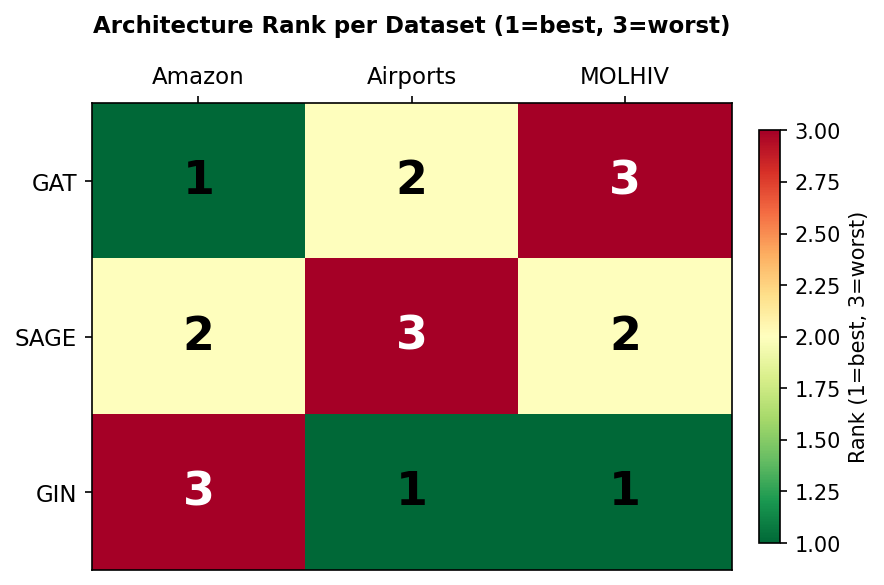
\includegraphics[width=0.49\columnwidth]{figures/cross_dataset_rank.png}%
\hfill
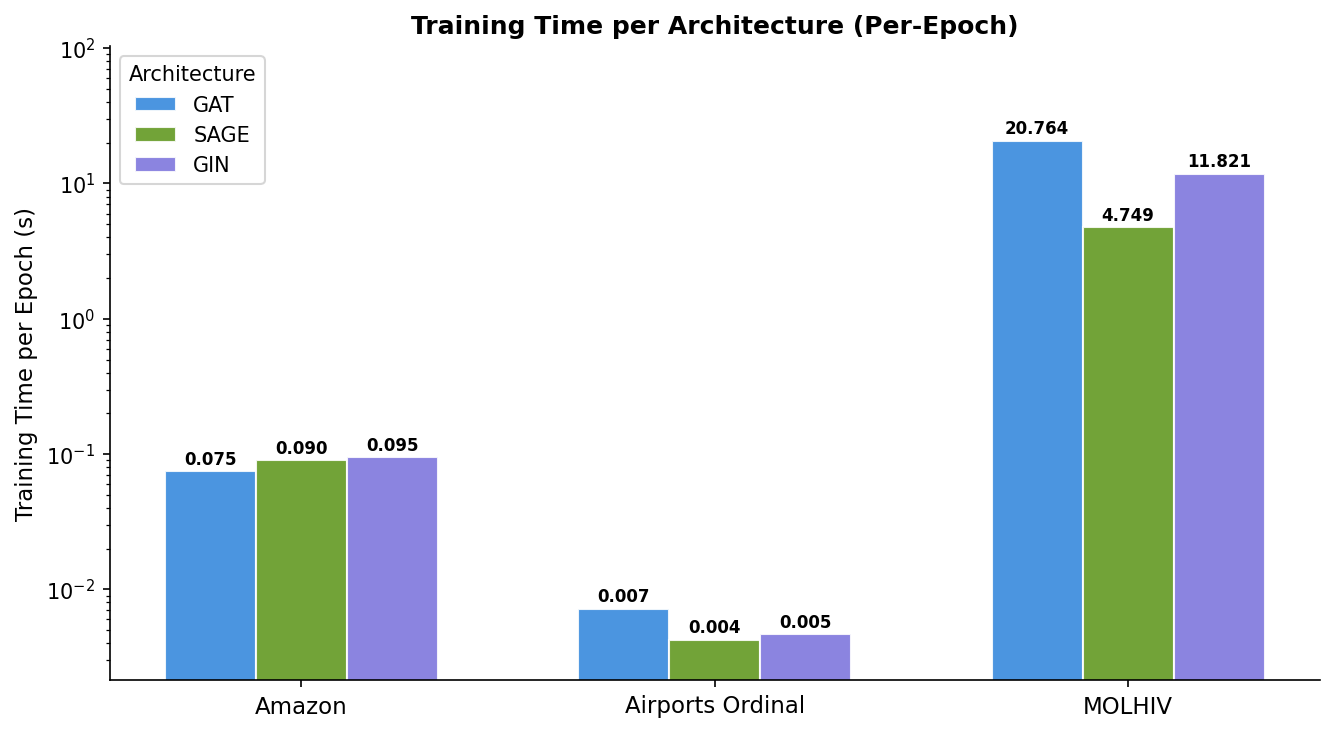
\includegraphics[width=0.49\columnwidth]{figures/cross_dataset_time.png}
\caption{Left: rank heatmap across datasets (green=best, red=worst). Right: training time in seconds per architecture per dataset. MOLHIV training times ($>$1,000 s) dwarf node-level tasks ($<$20 s) due to the 41,127-graph scale.}
\label{fig:cross_rank_time}
\end{figure}

\subsection{Architecture-Level Analysis}

Table~\ref{tab:cross} and Fig.~\ref{fig:cross_rank_time} synthesise the relative rankings and training efficiencies of the three architectures. Fig.~\ref{fig:summary} provides a unified view of their primary performance metrics on each respective benchmark.

\textbf{GIN} is the most consistently strong architecture overall with a rank sum of 5 (rank 1 on Airports and MOLHIV, rank 3 on Amazon). Its sum aggregator is theoretically the most expressive under the Weisfeiler-Lehman (WL) graph isomorphism test. This expressivity translates directly to ordinal regression performance---its ordinal kappa of 0.5758 is the highest among GNNs on Airports. On MOLHIV, its native bond-feature integration allows it to achieve the highest ROC-AUC of 0.7842. However, on Amazon its sum aggregation conflates category signals from high-degree hub nodes, leading to third place.

\textbf{GAT} ranks second overall (rank sum = 6) with a strong profile: rank 1 on Amazon (90.99\%), rank 2 on Airports (kappa 0.5069), but rank 3 on MOLHIV (0.7761 ROC-AUC). On Amazon, its attention mechanism most effectively differentiates informative from noisy co-purchase edges. On Airports, attention's edge-selectivity is less critical than aggregation-function expressivity.

\textbf{GraphSAGE} ranks third overall (rank sum = 7): second on Amazon (90.80\%) and MOLHIV (0.7785 ROC-AUC), but third on Airports (kappa 0.3773). Its mean aggregator excels at large-scale node classification and molecular screening but fails to capture the fine ordinal structure of the Airports task, where the monotonic degree--activity relationship requires sum-type aggregation to accumulate hub-centric connectivity evidence. As highlighted in Fig.~\ref{fig:cross_rank_time}, the most striking GraphSAGE finding is its MOLHIV efficiency: without bond features, it trails GIN by only 0.0057 ROC-AUC while using fewer than half as many parameters and demanding significantly less compute time.

\subsection{Ordinal Regression Lesson}

The Airports experiment reveals a nuanced lesson about loss function choice. While mean kappa delta across architectures is $-0.008$ (marginally favouring classification), the ordinal MSE loss completely eliminates catastrophic regional-to-hub misclassifications (2.381 pp reduction). This suggests that aggregate metrics such as kappa can mask qualitatively different error distributions: a practitioner who cares about the \emph{worst-case} error---predicting a regional airport as a major international hub---should strongly prefer the ordinal formulation even when classification wins marginally on kappa.

\subsection{Practitioner Decision Guide}

\begin{itemize}
    \item \textbf{Choose GAT} when edge-level attention matters (heterogeneous or noisy graphs with varying link quality) and edge features are available; it is the most robust overall architecture across all three task types.
    \item \textbf{Choose GraphSAGE} for large-scale tasks with tight parameter or compute budgets; it delivers competitive performance (within 0.2 pp of GAT on Amazon, within 0.002 ROC of GAT on MOLHIV) at less than half the parameter count.
    \item \textbf{Choose GIN} when the task is inherently ordinal or when neighbourhood multiset distinctiveness is critical (e.g., distinguishing hub-vs-spoke connectivity patterns); its sum aggregator maximises WL-expressiveness.
    \item \textbf{Prefer ordinal MSE over CrossEntropy} whenever class labels carry natural ordering---the quadratic gradient penalty eliminates extreme misclassification at negligible cost to average kappa, and may be decisive in safety-critical applications such as infrastructure planning.
\end{itemize}

% ─────────────────────────────────────────────────────────────────────────────
\section{Conclusion}
% ─────────────────────────────────────────────────────────────────────────────

This paper presents an empirical comparison of GAT, GraphSAGE, and GIN across three heterogeneous graph-learning benchmarks. GAT achieves the best test accuracy of 90.99\% on Amazon Computers, while GIN achieves the highest ROC-AUC of 0.7842 on OGBG-MOLHIV and leads on the Airports ordinal task (kappa = 0.5758), ranking first overall with a cross-dataset rank sum of 5. GIN's ordinal MSE formulation eliminates all catastrophic regional-to-hub misclassifications, reducing the catastrophic error rate from 2.381\% to 0.000\% relative to CrossEntropyLoss. Ablation studies on MOLHIV confirm that both atom features and bond topology are necessary: removing either modality costs 0.127--0.267 ROC-AUC across architectures, with GraphSAGE (structure-only, 0.5112 ROC) experiencing the most severe degradation. The t-SNE visualisations reveal that all three models place active-molecule clusters internally within the inactive manifold, reflecting the extreme 25.71:1 class imbalance; GraphSAGE is most balanced with 92.24\% active recall and only 8.47\% inactive misclassification. Finally, the degree heuristic ($\kappa = 0.6318$) outperforms all GNNs on Airports, underscoring that when structural position is the sole meaningful signal and the feature matrix carries no semantic content, simple structural baselines remain competitive. Future work should explore heterogeneous graph transformers that jointly attend over atom, bond, and scaffold-level representations to further close the gap on molecular HIV inhibition prediction.

% ─────────────────────────────────────────────────────────────────────────────
\begin{thebibliography}{9}

\bibitem{gilmer2017}
J.\ Gilmer, S.\ S.\ Sch\"{u}tt, F.\ Brockherde, G.\ E.\ Dahl, and K.\ T.\ M\"{u}ller,
``Neural message passing for quantum chemistry,''
in \textit{Proc.\ ICML}, 2017, pp.\ 1263--1272.

\bibitem{velickovic2018}
P.\ Veli\v{c}kovi\'{c}, G.\ Cucurull, A.\ Casanova, A.\ Romero, P.\ Lio, and Y.\ Bengio,
``Graph attention networks,''
in \textit{Proc.\ ICLR}, 2018.

\bibitem{hamilton2017}
W.\ L.\ Hamilton, Z.\ Ying, and J.\ Leskovec,
``Inductive representation learning on large graphs,''
in \textit{Proc.\ NeurIPS}, 2017, pp.\ 1024--1034.

\bibitem{xu2019}
K.\ Xu, W.\ Hu, J.\ Leskovec, and S.\ Jegelka,
``How powerful are graph neural networks?''
in \textit{Proc.\ ICLR}, 2019.

\bibitem{kipf2017}
T.\ N.\ Kipf and M.\ Welling,
``Semi-supervised classification with graph convolutional networks,''
in \textit{Proc.\ ICLR}, 2017.

\bibitem{brody2022}
S.\ Brody, U.\ Alon, and E.\ Yahav,
``How attentive are graph attention networks?''
in \textit{Proc.\ ICLR}, 2022.

\bibitem{shchur2018}
O.\ Shchur, M.\ Mumme, A.\ Bojchevski, and S.\ G\"{u}nnemann,
``Pitfalls of graph neural network evaluation,''
\textit{arXiv preprint arXiv:1811.05868}, 2018.

\bibitem{ribeiro2017}
L.\ F.\ R.\ Ribeiro, P.\ H.\ P.\ Saverese, and D.\ R.\ Figueiredo,
``struc2vec: Learning node representations from structural identity,''
in \textit{Proc.\ KDD}, 2017, pp.\ 385--394.

\bibitem{hu2020}
W.\ Hu, M.\ Fey, M.\ Zitnik, Y.\ Dong, H.\ Ren, B.\ Liu, M.\ Catasta, and J.\ Leskovec,
``Open graph benchmark: Datasets for machine learning on graphs,''
in \textit{Proc.\ NeurIPS}, 2020.

\end{thebibliography}

\end{document}
